\documentclass[10pt,twoside,openright]{memoir}
\usepackage[paperwidth=4.25in, paperheight=6.875in]{geometry}
\usepackage[utf8]{inputenc} % If utf8 encoding                                  
\usepackage[T1]{fontenc}    %                                                   
\usepackage[english]{babel} % English please                                    
\usepackage[final]{microtype} % Less badboxes 
\usepackage{caption}
\usepackage{graphicx}
\usepackage{rotating}
\usepackage{tikz}
\usepackage{eso-pic,xcolor,lipsum,calc}
\usepackage{helvet}



%\renewcommand{\familydefault}{\sfdefault}


%%% BEGIN DOCUMENT

\begin{document}


\pagenumbering{gobble}


\begin{vplace}
\begin{center}
  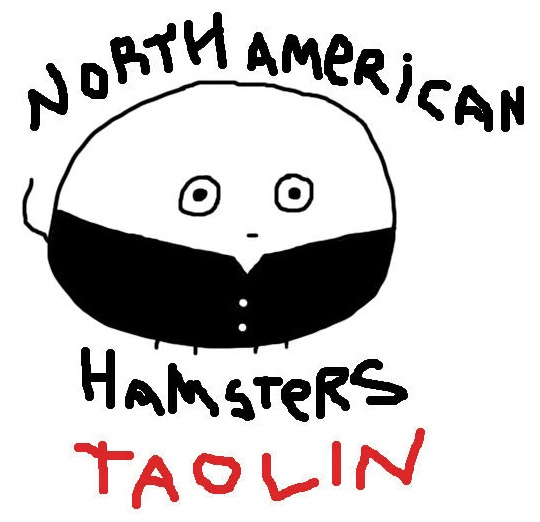
\includegraphics[width=2in]{img/cover}
\end{center}
\end{vplace}

\pagebreak
\mbox{}


\pagebreak
\mbox{}


\pagebreak

\begin{vplace}
\noindent
In {\em North American Hamsters}, a collection of short essays gathered and 
printed without the consent of the author, Tao Lin takes the reader on a
whimsical, action-packed safari that eschews big-game animals for an
oft-overlooked rodent: the humble hamster.

\begin{center}
\textbf{Praise for Tao Lin}
\\[1em]

``I want to download the new Tao Lin and read it by bike light in a Mongolian
yurt.''\\
--Allison Reibel

\vspace{1em}

``As Tao Lin would say, I'm fucked.'' \\
--Allison Reibel
\end{center}
\end{vplace}

\end{document}
